% \begin{frame}
% \begin{center}
% TODO \cite{abbott2005data}
% \end{center}
% \end{frame}

\begin{frame}
\begin{center}
The term zipper is a colloquial that is used to describe n-hole contexts into a data structure; most often \lstinline{n=1}.
\end{center}
\end{frame}

\begin{frame}
\begin{center}
That is, a data structure that has a hole or pointer focussed on a specific element.
\end{center}
\end{frame}

\begin{frame}
\begin{center}
An important property of a zipper is an ability to efficiently traverse to and modify neighbours.
\end{center}
\end{frame}

\begin{frame}
\begin{block}{Loosely speaking}
\begin{center}
Take any data structure and walk to any element (1-hole) on it.
\end{center}
\end{block}
\begin{center}
Now look around you. What do you see?
\end{center}
\end{frame}

\begin{frame}
\begin{block}{For example}
\begin{center}
Here is the list one to ten
\end{center}
\end{block}
\begin{center}
\lstinline{[1,2,3,4,5,6,7,8,9,10]}
\end{center}
\end{frame}

\begin{frame}
\begin{block}{For example}
\begin{center}
Here is a depiction of a physical list one to ten
\end{center}
\end{block}
\begin{center}
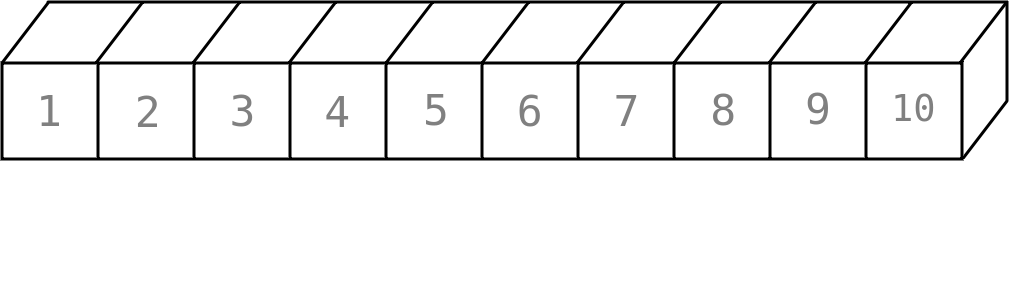
\includegraphics[width=1.25\textheight]{image/list1-10.png}
\end{center}
\end{frame}

\begin{frame}
\begin{block}{For example}
\begin{center}
Let's move to the element containing \lstinline{7}
\end{center}
\end{block}
\begin{center}
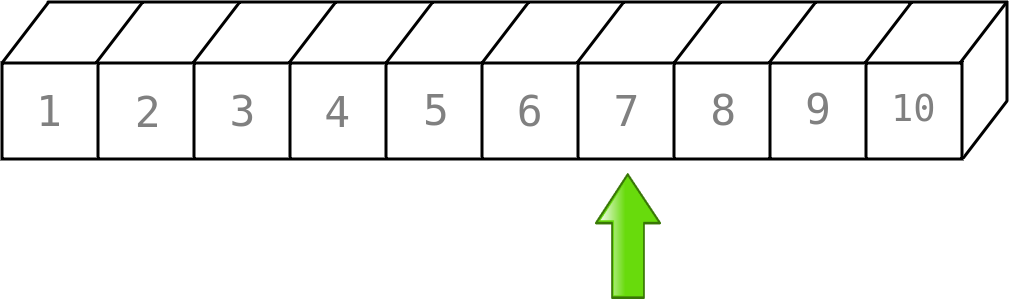
\includegraphics[width=1.25\textheight]{image/list1-10-arrow7.png}
\end{center}
\end{frame}

\begin{frame}
\begin{block}{List zipper}
\begin{center}
and look around us
\end{center}
\end{block}
\begin{center}
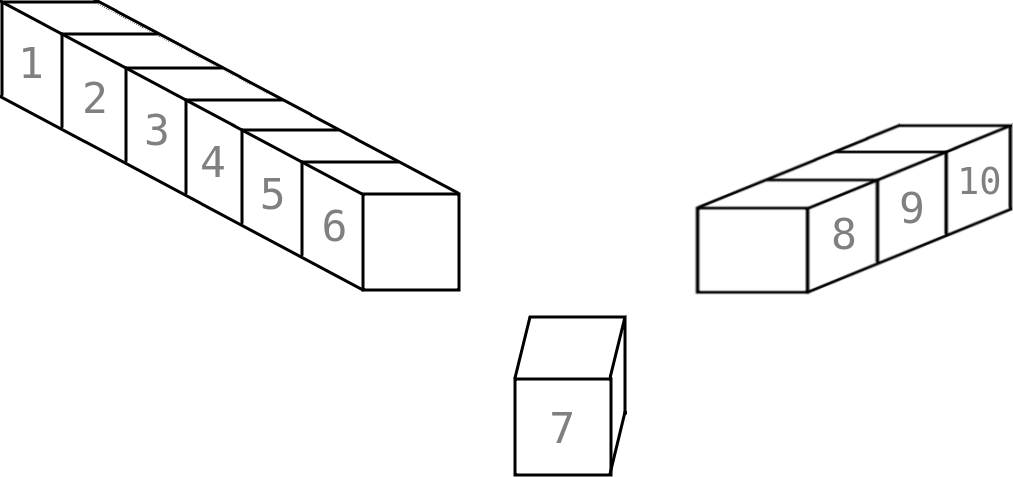
\includegraphics[width=1.25\textheight]{image/listzipper1-10.png}
\end{center}
\begin{center}
\lstinline{([6,5,4,3,2,1], 7, [8,9,10])}
\end{center}
\end{frame}

\begin{frame}
\begin{block}{List zipper}
\begin{center}
and look around us
\end{center}
\end{block}
\begin{center}
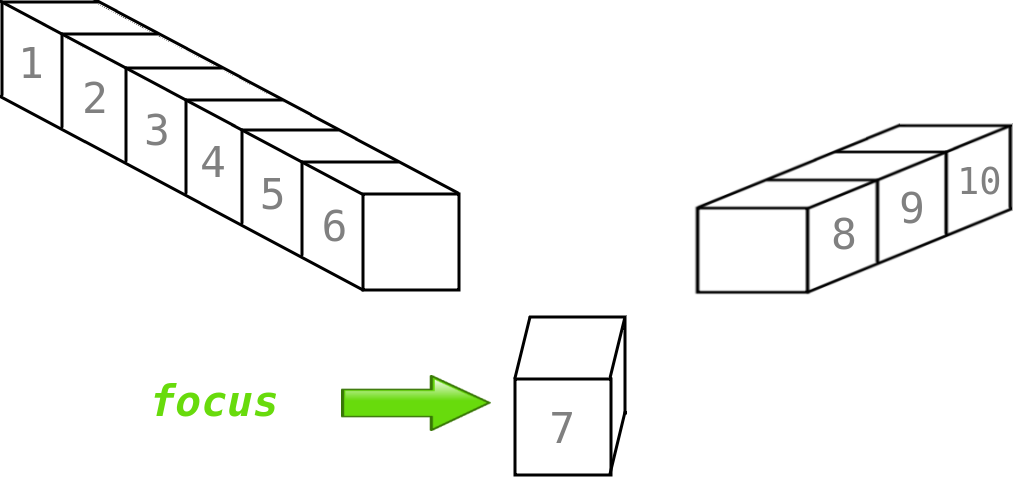
\includegraphics[width=1.25\textheight]{image/listzipper1-10-focus.png}
\end{center}
\begin{center}
\lstinline{([6,5,4,3,2,1], 7, [8,9,10])}
\end{center}
\end{frame}

\begin{frame}[fragile]
\begin{block}{List zipper}
\begin{center}
We can easily move to our neighbours in O(1) time
\end{center}
\end{block}
\begin{center}
\begin{lstlisting}[style=haskell]
listz =
  ([6,5,4,3,2,1], 7, [8,9,10])
  
moveLeft listz =
  ([5,4,3,2,1], 6, [7,8,9,10])
\end{lstlisting}
\end{center}
\end{frame}

\begin{frame}[fragile]
\begin{block}{List zipper}
\begin{center}
The zipper for \lstinline{[a]} is \lstinline{([a], a, [a])}
\end{center}
\end{block}
\begin{center}
\begin{lstlisting}[style=haskell]
data ListZipper a =
  ListZipper [a] a [a]
\end{lstlisting}
\end{center}
\end{frame}

\begin{frame}[fragile]
\begin{block}{List zipper}
\begin{center}
Some useful operations on a list zipper:
\begin{itemize}
  \item \tiny{\lstinline{moveLeft/Right :: ListZipper a -> Maybe (ListZipper a)}}
  \item \tiny{\lstinline{findLeft/Right :: (a -> Bool) -> ListZipper a -> Maybe (ListZipper a)}}
  \item \tiny{\lstinline{modify :: (a -> a) -> ListZipper a -> ListZipper a}}
  \item \tiny{\lstinline{delete :: ListZipper a -> Maybe (ListZipper a)}}
\end{itemize}
\end{center}
\end{block}
\end{frame}

\begin{frame}[fragile]
\begin{block}{Multi-way Tree}
\begin{center}
How about a multi-way tree?
\end{center}
\end{block}
\begin{center}
\begin{lstlisting}[style=haskell]
data Tree a =
  Tree a [Tree a]
\end{lstlisting}
\end{center}
\end{frame}

\begin{frame}[fragile]
\begin{block}{What if we stand on an element and look around?}
\begin{center}
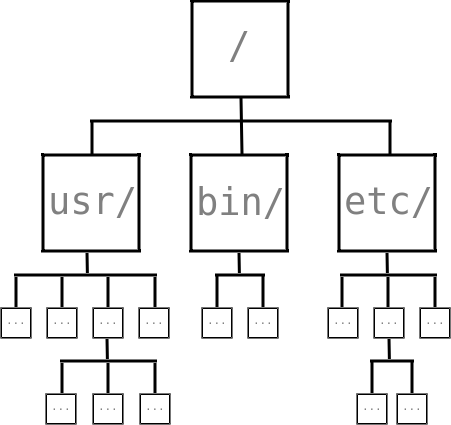
\includegraphics[width=0.60\textheight]{image/rosetree.png}
\end{center}
\end{block}
\end{frame}

\begin{frame}[fragile]
\begin{block}{\lstinline{leftSiblings :: ?}}
\begin{center}
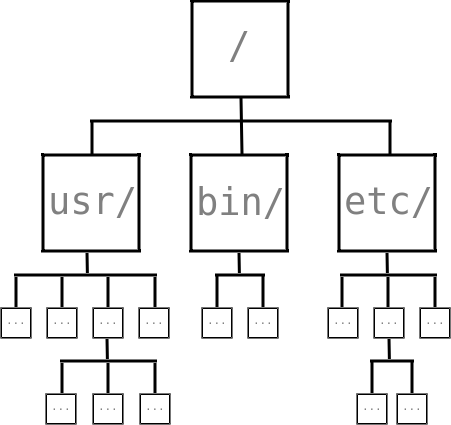
\includegraphics[width=0.60\textheight]{image/rosetree.png}
\end{center}
\end{block}
\end{frame}

\begin{frame}[fragile]
\begin{block}{\lstinline{leftSiblings :: [Tree a]}}
\begin{center}
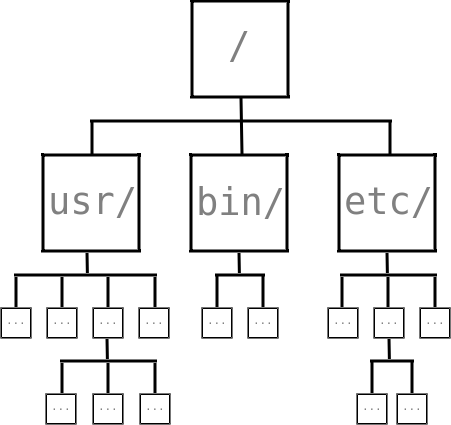
\includegraphics[width=0.60\textheight]{image/rosetree.png}
\end{center}
\end{block}
\end{frame}

\begin{frame}[fragile]
\begin{block}{\lstinline{rightSiblings :: [Tree a]}}
\begin{center}
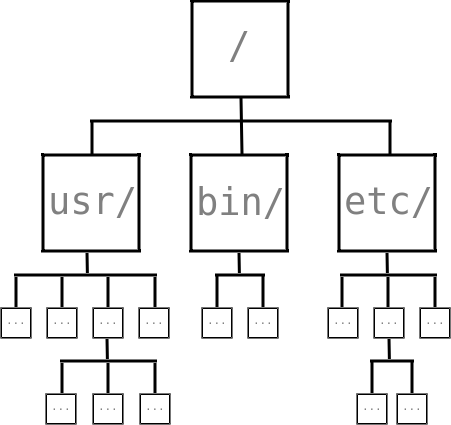
\includegraphics[width=0.60\textheight]{image/rosetree.png}
\end{center}
\end{block}
\end{frame}

\begin{frame}[fragile]
\begin{block}{\lstinline{focus :: ?}}
\begin{center}
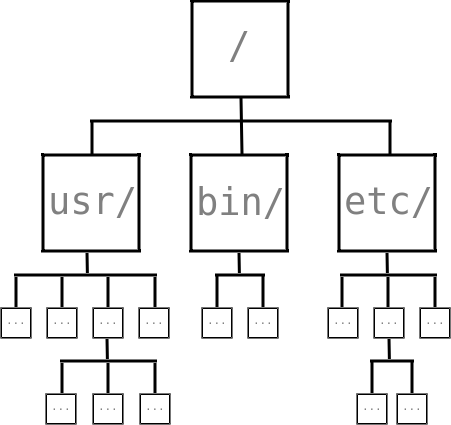
\includegraphics[width=0.60\textheight]{image/rosetree.png}
\end{center}
\end{block}
\end{frame}

\begin{frame}[fragile]
\begin{block}{\lstinline{focus :: a}}
\begin{center}
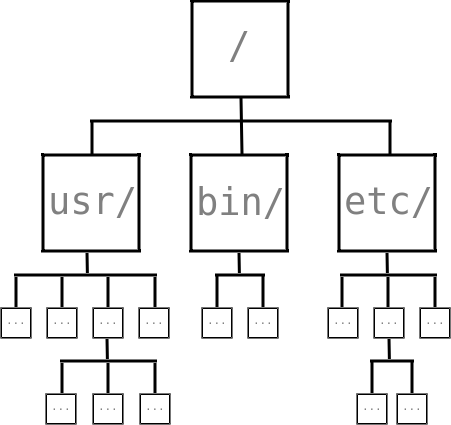
\includegraphics[width=0.60\textheight]{image/rosetree.png}
\end{center}
\end{block}
\end{frame}

\begin{frame}[fragile]
\begin{block}{\lstinline{children :: ?}}
\begin{center}
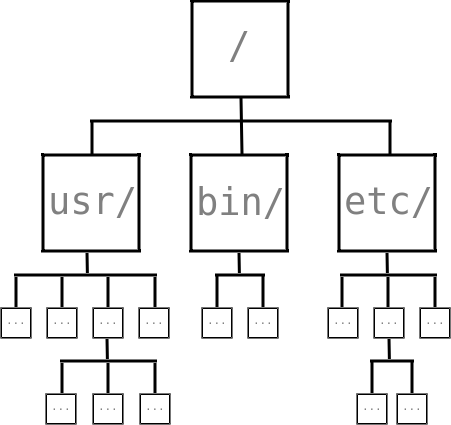
\includegraphics[width=0.60\textheight]{image/rosetree.png}
\end{center}
\end{block}
\end{frame}

\begin{frame}[fragile]
\begin{block}{\lstinline{children :: [Tree a]}}
\begin{center}
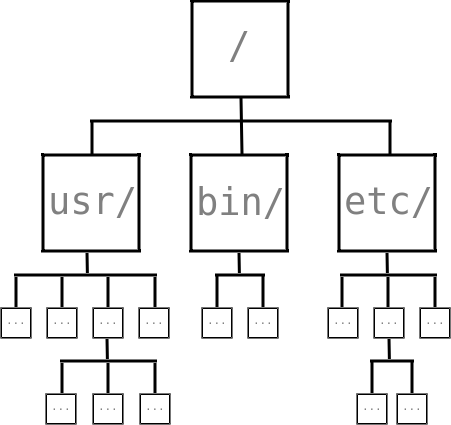
\includegraphics[width=0.60\textheight]{image/rosetree.png}
\end{center}
\end{block}
\end{frame}

\begin{frame}[fragile]
\begin{block}{\lstinline{parents :: ?}}
\begin{center}
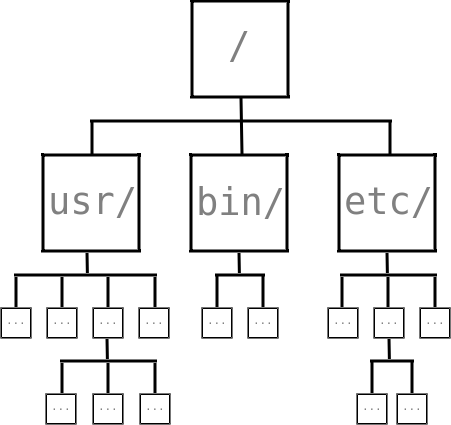
\includegraphics[width=0.60\textheight]{image/rosetree.png}
\end{center}
\end{block}
\end{frame}

\begin{frame}[fragile]
\begin{block}{\lstinline{parents :: [([Tree a], a, [Tree a])]}}
\begin{center}
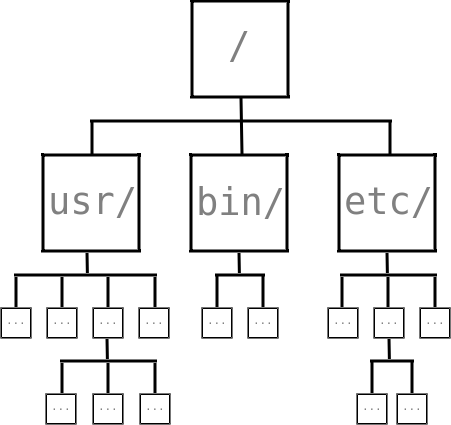
\includegraphics[width=0.60\textheight]{image/rosetree.png}
\end{center}
\end{block}
\end{frame}

\begin{frame}[fragile]
\begin{block}{The zipper for a multi-way tree is}
\begin{lstlisting}[style=haskell]
data TreeZipper a =
  TreeZipper
    [Tree a]                -- left siblings
    [Tree a]                -- right siblings
    a                       -- focus
    [Tree a]                -- children
    ([Tree a], a, [Tree a]) -- parents
\end{lstlisting}
\end{block}
\end{frame}

\begin{frame}[fragile]
\begin{block}{Tree zipper}
\begin{center}
Some useful operations on a tree zipper:
\begin{itemize}
  \item \tiny{\lstinline{moveParent/Child :: TreeZipper a -> Maybe (TreeZipper a)}}
  \item \tiny{\lstinline{moveLeft/Right :: TreeZipper a -> Maybe (TreeZipper a)}}
  \item \tiny{\lstinline{find :: (a -> Bool) -> TreeZipper a -> Maybe (TreeZipper a)}}
  \item \tiny{\lstinline{all :: (a -> Bool) -> TreeZipper a -> Bool}}
  \item \tiny{\lstinline{modify :: (a -> a) -> TreeZipper a -> TreeZipper a}}
  \item \tiny{\lstinline{modifyTree :: (Tree a -> Tree a) -> TreeZipper a -> TreeZipper a}}
  \item \tiny{\lstinline{insertSiblingLeft/Right :: Tree a -> TreeZipper a -> TreeZipper a}}
\end{itemize}
\end{center}
\end{block}
\end{frame}

\begin{frame}[fragile]
\begin{block}{Other zippers}
\begin{center}
Some other data structures have useful zippers:
\begin{itemize}
  \item JSON
  \item CSV
  \item ASN.1
  \item text editors
  \item Pilot logbook
  \item \emph{many more!}
\end{itemize}
\end{center}
\end{block}
\end{frame}
